% Generated by experiments/paper/fig_lorenz.py; do not edit.
\begin{figure*}[t]
\centering
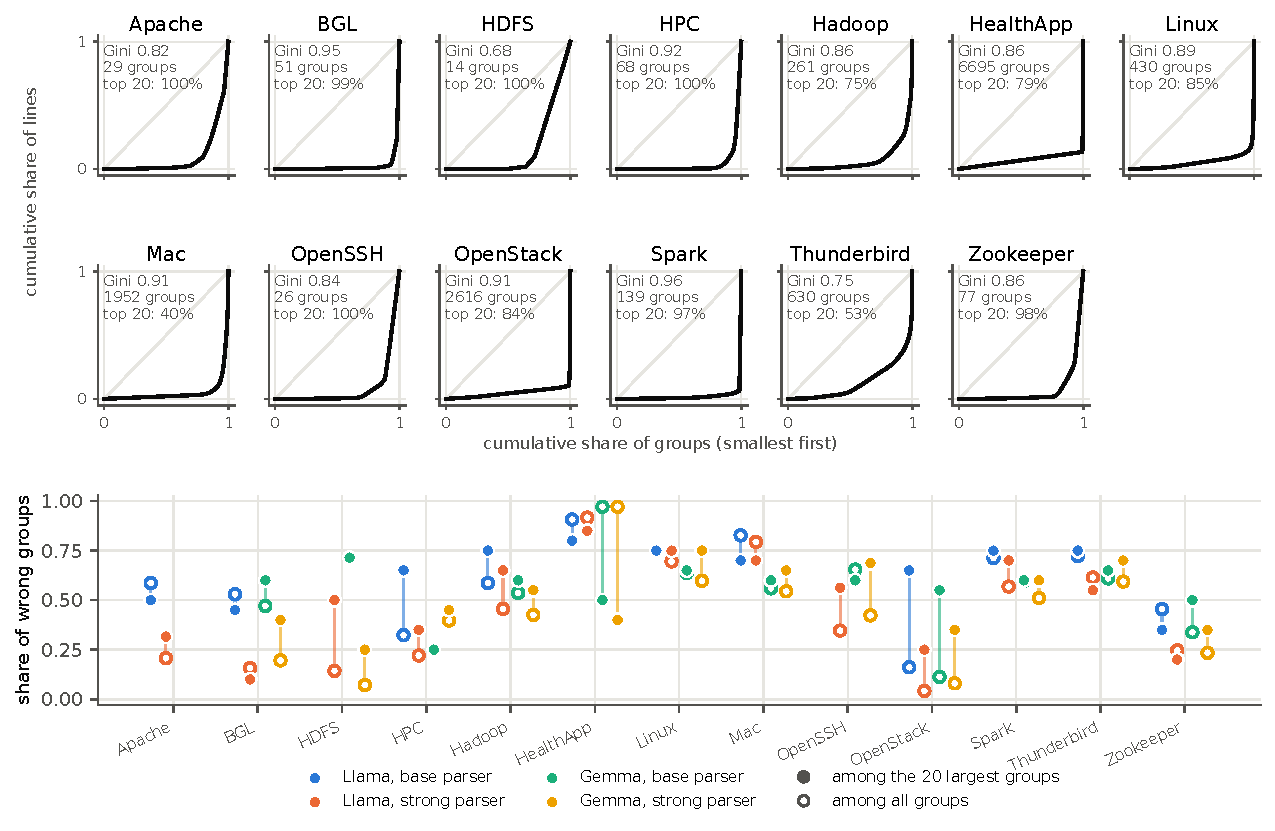
\includegraphics[width=\textwidth]{figures/lorenz.pdf}
\caption{Why reviewing the most frequent groups first nearly matches the oracle. Top: Lorenz curves of Drain group sizes over each system's first 50,000 lines (Loghub-2.0 settings); the 20 largest groups hold most lines. Bottom: share of wrong groups (cached template differs from the first line's ground truth) among the 20 largest groups (filled) and among all groups (hollow), per model and parser (base: zero-shot greedy; strong: kNN demonstrations + AdaParser corrector + 10 verified seed groups, which are excluded from the 20).}
\label{fig:lorenz}
\end{figure*}
